\documentclass[xcolor=table,dvipsnames]{beamer}
  \definecolor{lg}{rgb}{.85,.85,.85}
  \usepackage{graphicx}

  \usecolortheme[named=teal]{structure}
  % \usetheme[compact]{Singapore}
  \setbeamerfont{frametitle}{size = {\large}, family=\rmfamily}
  \setbeamertemplate{navigation symbols}{}
  % packages for extra math symbols
  \usepackage{amsthm, amsmath, amssymb} 

  % I like these fonts better
  \usepackage{mathpazo}

  \usepackage{tikz}
  \usetikzlibrary{arrows}
  \usetikzlibrary{decorations.markings}
  \tikzstyle{dot}=[circle, inner sep=.4mm, draw=black, outer sep=2mm, fill=black]
  \tikzstyle{gdot}=[circle, inner sep=.4mm, draw=black!25, outer sep=2mm,
                    fill=black!25]
  \tikzstyle{odot}=[circle, inner sep=.4mm, draw=black, outer sep=2mm]
  \pgfdeclarelayer{bg}
  \pgfsetlayers{bg,main}


  \usepackage{pgfplots}
  \pgfplotsset{compat=1.8}

  \DeclareMathOperator{\Av}{Av}

  \newcommand{\num}{\nu}
  \newcommand{\ds}{\displaystyle}
  \newcommand{\ra}{\rightarrow}
  \newcommand{\R}{\mathbb{R}}
  \newcommand{\sg}{\sigma}
  \renewcommand{\S}{\mathfrak{S}}
  \newcommand{\C}{\mathcal{C}}

  \newcommand{\Ex}[1]{\mathbb{E}\left[ #1 \right]}


  

% ===================================================================== %
\begin{document}


\title[Deflatability]%
  {\Large \rm Deflatability in Permutation Classes}

\author{Cheyne Homberger \\ {\small University of Maryland, Baltimore County}}

\date{\small AMS Eastern Sectional Meeting \\ 
        Georgetown University \\ 
        \today \\[2pc]
        (Joint work with Michael Albert, Mike Atkinson, and Jay Pantone)
  }


\begin{frame}
  \titlepage
\end{frame}




% \begin{frame} \frametitle{Permutations}
%   \pause
%   \begin{block}{Definition}
%     An \emph{permutation of length $n$} is a bijection from the set $[n] = \{1,
%     2, \dots n\}$ to itself. The \emph{one-line notation} for a permutation
%     $\pi$ is 
%     $$ \pi = \pi(1) \pi(2) \dots \pi(n). $$
% 
%     The set of all permutations of length $n$ is denoted $\S_n$. 
%   \end{block}
%   \pause
%   \vspace{1pc}
% 
%   \begin{center}
%   \begin{block}{Examples}
%     \begin{itemize}
%       \item The sequence $\pi = 5172643$ is a permutation of length $7$. 
%       \pause
%       \item The six permutations of length $3$ are 
%         $$ \S_3 = \{123, 132, 213, 231, 312, 321\}. $$
%     \end{itemize}
%   \end{block}
%   \end{center}
% \end{frame}

\begin{frame} \frametitle{Plotting Permutations}
  \begin{block}{Definition}
    If $\pi$ is a permutation of length $n$, then the \emph{plot}
    of $\pi$ is the set of points 
    $$ \{ (1, \pi(1)), (2, \pi(2)), \cdots (n, \pi(n)) \} \subset \mathbb{R}^2 $$
  \end{block}

  \pause 
  \begin{center}
  \begin{tikzpicture}[scale = .5,
                      dot/.style={circle, fill=teal, inner sep=.5mm}]
    \draw[<->] (0,6) -- (0,0) -- (6,0);
    \foreach \y [count = \x] in {3,5,1,4,2}{
    % \node[dot, label=210:{{\tiny $(\x,\y)$}}] at (\x,\y) {};
      \node[dot] at (\x,\y) {};
      \draw (\x,-.25) -- (\x, .25);
      \draw (-.25, \x) -- (.25, \x);
    }
    \pause
    {\scriptsize
    \node[anchor=south west] at (1,3) {3};
    \pause
    \node[anchor=south west] at (2,5) {5};
    \pause
    \node[anchor=south west] at (3,1) {1};
    \pause
    \node[anchor=south west] at (4,4) {4};
    \pause
    \node[anchor=south west] at (5,2) {2};
    }
  \end{tikzpicture}
  \end{center}
  \uncover<2->{
  $$ \pi = 35142 $$
  }
\end{frame}

\begin{frame} \frametitle{Dots on a Plane} 
  \only<1->{
  \begin{block}{Definition} 
    Let $A$ and $B$ be two sets of $n$ points in $\R^2$, each with the property
    that no two points lie on the same horizontal or vertical line. \\
    Say that $A$ is \emph{order isomorphic} to $B$ (denoted $A \sim B$) if $A$
    can be transformed into $B$ by stretching, contracting, and translating the
    axes horizontally and vertically.
  \end{block}
  }
  
  \vspace{.5pc}

  \pause 

  \begin{block}{Example}
    \vspace{1pc}
    \begin{tikzpicture}[scale = .45,
                        dot/.style={circle, fill=teal, inner sep=.5mm}]
      \node[dot] at (1,3.5) {};
      \node[dot] at (1.3,4.5) {};
      \node[dot] at (3,.5) {};
      \node[dot] at (3.4,4) {};
      \node[dot] at (5,1) {};
      {\scriptsize
      \uncover<5->{\node[anchor=south west] at (3,.5) {1};}
      \uncover<6->{\node[anchor=south west] at (5,1) {2};}
      \uncover<7->{\node[anchor=south west] at (1,3.5) {3};}
      \uncover<8->{\node[anchor=south west] at (3.4,4) {4};}
      \uncover<9->{\node[anchor=south west] at (1.3,4.5) {5};}
      }
    \end{tikzpicture}
    \hspace{1pc}
    \raisebox{2.5pc}{$\sim$}
    \hspace{1pc}
    \begin{tikzpicture}[scale = .45,
                        dot/.style={circle, fill=teal, inner sep=.5mm}]
      \node[dot] at (1,2) {};
      \node[dot] at (2.5,5) {};
      \node[dot] at (3,1) {};
      \node[dot] at (3.5,4) {};
      \node[dot] at (5,1.5) {};
      {\scriptsize
      \uncover<5->{\node[anchor=south west] at (3,1) {1};}
      \uncover<6->{\node[anchor=south west] at (5,1.5) {2};}
      \uncover<7->{\node[anchor=south west] at (1,2) {3};}
      \uncover<8->{\node[anchor=south west] at (3.5,4) {4};}
      \uncover<9->{\node[anchor=south west] at (2.5,5) {5};}
      }
    \end{tikzpicture}
    \hspace{1pc}
    \pause
    \raisebox{2.5pc}{$\sim$}
    \hspace{1pc}
    \begin{tikzpicture}[scale = .45,
                        dot/.style={circle, fill=teal, inner sep=.5mm}]
      \foreach \y [count = \x] in {3,5,1,4,2}
      \node[dot] at (\x,\y) {};
      {\scriptsize
      \uncover<5->{\node[anchor=south west] at (3,1) {1};}
      \uncover<6->{\node[anchor=south west] at (5,2) {2};}
      \uncover<7->{\node[anchor=south west] at (1,3) {3};}
      \uncover<8->{\node[anchor=south west] at (4,4) {4};}
      \uncover<9->{\node[anchor=south west] at (2,5) {5};}
      }
    \end{tikzpicture}

    \pause
    \vspace{1pc}
    { \hfill $\pi = 35142$ \hspace{2pc}}
  \end{block}
\end{frame}

\begin{frame} \frametitle{Permutation Patterns} 
  \begin{block}{Definition}
    Let $\pi = \pi(1) \pi(2) \cdots \pi(n)$ and 
    $\sg = \sg(1) \sg(2) \cdots \sg(k)$ be two permutations.
    $\pi$ \emph{contains $\sg$ as a pattern} (written $\sg \prec
    \pi$) if there is some subsequence $\pi(i_1) \pi(i_2) \ldots \pi(i_k)$
    which is order isomorphic to the entries of $\sg$ (i.e.,
    $\pi(i_j) < \pi(i_k)$ if and only if $\sg(j) < \sg(k)$).  
  \end{block}
  \pause 

  \vspace{1pc}

  \begin{center}
  \begin{tikzpicture}[scale = .5,
                      dot/.style={circle, fill=teal, inner sep=.5mm}]
    \node[dot] at (1,2) {};
    \node[dot] at (2,1) {};
    \node[dot] at (3,3) {};
    \node[] at (1,0) {};
  \end{tikzpicture}
  %
    \hspace{1pc}
    \raisebox{2pc}{$\prec$}
    \hspace{1pc}
  %
  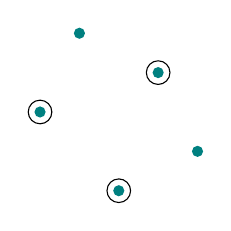
\begin{tikzpicture}[scale = .5,
                      dot/.style={circle, fill=teal, inner sep=.5mm}]
    \foreach \y [count = \x] in {3,5,1,4,2}
    \node[dot] at (\x,\y) {};
    \uncover<3>{
      \draw (1,3) circle (3mm);
      \draw (3,1) circle (3mm);
      \draw (4,4) circle (3mm);
    }
      
  \end{tikzpicture}
  \end{center}

  \vspace{1pc}

  $$ 213 \qquad \prec \qquad 
    \only<3>{\mathbf}35\only<3>{\mathbf}1\only<3>{\mathbf}42 $$
\end{frame}


\begin{frame}{Simplicity} 
  \begin{block}{Definition}
    An \emph{interval} of a permutation $\pi = \pi_1 \pi_2 \dots \pi_n$ is a
    sequence of consecutive entries $\pi_i \pi_{i+1} \dots \pi_{i+k}$ whose
    values form a sequence of consecutive integers. Intervals of size $1$ and
    $n$ are said to be \emph{trivial}. 
  \end{block}

  \pause

  \begin{center}
  \begin{tikzpicture}[scale=.4]
    \foreach \y [count = \x] in {9,2, 4,6,5,10,3,7, 1, 8}
      \draw[fill=black] (\x, \y) circle (2mm);
    \uncover<4->{
      \draw (2.5, 3.5) -- (2.5, 6.5) -- (5.5, 6.5) -- (5.5, 3.5) -- cycle;
    }
    \uncover<5>{
      \draw (1, 3.5) -- (10, 3.5);
      \draw (1, 6.5) -- (10, 6.5);
      \draw (2.5, 1) -- (2.5, 10);
      \draw (5.5, 1) -- (5.5, 10);
    }
    \only<3>{\node at (4.5,-1.2) {$\pi = 9\ 2\ 4\ 6\ 5\ 10\ 3\ 7\ 1\ 8$};}
    \only<4->{\node at (4.5,-1.2) 
      {$\pi = 9\ 2 \boxed{4\ 6\ 5} 10\ 3\ 7\ 1\ 8$};}
    \node at (5,-2) {};
    \node at (-2,-2) {};
  \end{tikzpicture}
  \end{center}

\end{frame}

\begin{frame}{Simplicity}
  \begin{block}{Definition}
    A permutation is said to be \emph{simple} if it has no non-trivial
    intervals.
  \end{block}
  \pause 
  \begin{center}
  \begin{tikzpicture}[scale=.4]
    \foreach \x/\y  in {1/9,2/2,6/10,7/3,8/7, 9/1, 10/8}
      \draw[fill=black] (\x, \y) circle (2mm);

    \only<2>{\foreach \x/\y  in {3/4,4/6,5/5}
      \draw[fill=black] (\x, \y) circle (2mm);
    }
    \only<3->{
      \draw[fill=black] (4, 5) circle (2mm);
    }

    \only<2-3>{
    \draw (2.5, 3.5) -- (2.5, 6.5) -- (5.5, 6.5) -- (5.5, 3.5) -- cycle;
    \draw (1, 3.5) -- (10, 3.5);
    \draw (1, 6.5) -- (10, 6.5);
    \draw (2.5, 1) -- (2.5, 10);
    \draw (5.5, 1) -- (5.5, 10);
    }
    
    \only<2>{\node at (4.5,-1.2) {$\pi = 9\ 2 \boxed{4\ 6\ 5} 10\ 3\ 7\ 1\ 8$};}
    \only<3>{\node at (4.5,-1.2) {$\pi = 9\ 2 \boxed{5} 10\ 3\ 7\ 1\ 8$};}
    \only<4>{\node at (4.5,-1.2) {$\pi = 7\ 2\ 4\ 8\ 3\ 5\ 1\ 6$};}
    \node at (5,-2) {};
    \node at (-2,-2) {};
  \end{tikzpicture}
  \end{center}
\end{frame}

\begin{frame}{Inflations} 
  \begin{block}{Definition}
    For a permutation $\pi$ of length $n$, and permutations $\alpha_1,
    \alpha_2, \dots \alpha_n$, the \emph{inflation} of $\pi$ by $(\alpha_1,
    \alpha_2, \dots \alpha_n)$ (denoted $ \pi[\alpha_1, \alpha_2, \dots
    \alpha_n]$) is the permutation obtained by inflating the $i$th entry of
    $\pi$ by an interval isomorphic to $\alpha_i$. 
  \end{block}
  \uncover<3->{
  \begin{center}
    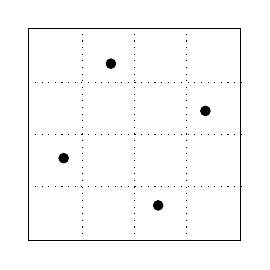
\begin{tikzpicture}[scale=.3]
      \draw (.5,.5) -- (9.5,.5) -- (9.5,9.5) -- (.5,9.5) -- cycle;
      \foreach \i in {2.8, 5, 7.2}{
        \draw[dotted] (.5,\i) -- (9.5, \i);
        \draw[dotted] (\i,.5) -- (\i, 9.5);
      }
      \draw[fill=black] (2, 4) circle (2mm);
      \draw[fill=black] (4, 8) circle (2mm);
      \draw[fill=black] (6, 2) circle (2mm);
      \draw[fill=black] (8,6) circle (2mm);
    \end{tikzpicture}
    }
    \uncover<4->{
    \hspace{1pc}
    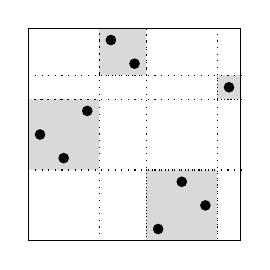
\begin{tikzpicture}[scale=.3]
      % \draw[fill=black!15] (.75,6.25)--(3.25,6.25)--(3.25,3.75)--(.75,3.75)--cycle;
      % \draw[fill=black!15] (3.75,9.25)--(5.25,9.25)--(5.25,7.75)--(3.75,7.75)--cycle;
      % \draw[fill=black!15] (5.75,3.25)--(8.25,3.25)--(8.25,.75)--(5.75,.75)--cycle;
      % \draw[fill=black!15] (8.75,7.25)--(9.25,7.25)--(9.25,6.75)--(8.75,6.75)--cycle;


      \draw[fill=black!15, dotted] 
          (.5,3.5)--(3.5,3.5)--(3.5,6.5)--(.5,6.5)--cycle;
      \draw[fill=black!15, dotted] 
          (3.5,7.5)--(5.5,7.5)--(5.5,9.5)--(3.5,9.5)--cycle;
      \draw[fill=black!15, dotted] 
          (5.5,.5)--(8.5,.5)--(8.5,3.5)--(5.5,3.5)--cycle;
      \draw[fill=black!15, dotted] 
          (8.5,6.5)--(9.5,6.5)--(9.5,7.5)--(8.5,7.5)--cycle;

      \draw (.5,.5) -- (9.5,.5) -- (9.5,9.5) -- (.5,9.5) -- cycle;
      \foreach \i in {3.5, 5.5, 8.5}{
        \draw[dotted] (\i,.5) -- (\i, 9.5);
      }
      \foreach \i in {3.5, 6.5, 7.5}{
        \draw[dotted] (.5,\i) -- (9.5, \i);
      }
      \foreach \y [count = \x] in {5,4,6,9,8,1,3,2,7}
        \draw[fill = black] (\x,\y) circle (2mm);
    \end{tikzpicture}
    }
    \hspace{1pc}
    \uncover<5->{
    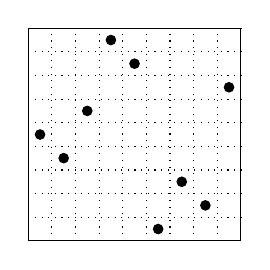
\begin{tikzpicture}[scale=.3]
    \draw (.5,.5) -- (9.5,.5) -- (9.5,9.5) -- (.5,9.5) -- cycle;

      \foreach \y [count = \x] in {5,4,6,9,8,1,3,2,7}{
        \draw[fill = black] (\x,\y) circle (2mm);
        \draw[dotted] (\x + 0.5, 0.5) -- (\x + 0.5, 9.5);
        \draw[dotted] (0.5, \x + 0.5) -- (9.5, \x + 0.5);
        }
  
    \end{tikzpicture}
    }
  \end{center}
  \uncover<2->{$$ 2413[213, 21, 132, 1] = 5\ 4\ 6\ 9\ 8\ 1\ 3\ 2\ 7$$}
\end{frame}

\begin{frame}{Substitution Decomposition}
  \begin{block}{Theorem (Albert and Atkinson)}
    Every permutation $\pi$ can be written as the inflation of a unique
    simple permutation $\sg$. Further, if $\sg$ has length at least four,
    then the inflating permutations are uniquely determined. 
  \end{block}
\end{frame}


\begin{frame}{Class Enumeration}
  \begin{block}{Idea}
    If we understand the simples within a permutation class, we can use them to 
    understand the class as a whole. 
  \end{block}
  \pause
  \begin{block}{Example}
    The only simple permutations in the class $\Av(132)$ are $\{1, 12, 21\}$. 
    Analyzing the ways in which these permutations can be inflated while 
    avoiding $132$ leads to a functional equation for the generating function 
    enumerating the class:
    $$ f = z + fz + z(f+1)f.$$
  \end{block}
  \pause
  \begin{block}{Example}
    The class $\Av(123)$ has infinitely many simple permutations, and cannot be 
    enumerated in this way. 
  \end{block}
  
\end{frame}



\newgeometry{margin=0mm}
\begin{frame} \frametitle{\hspace{28pt}Permutation Classes - Growth Rates} 
  \begin{center}
    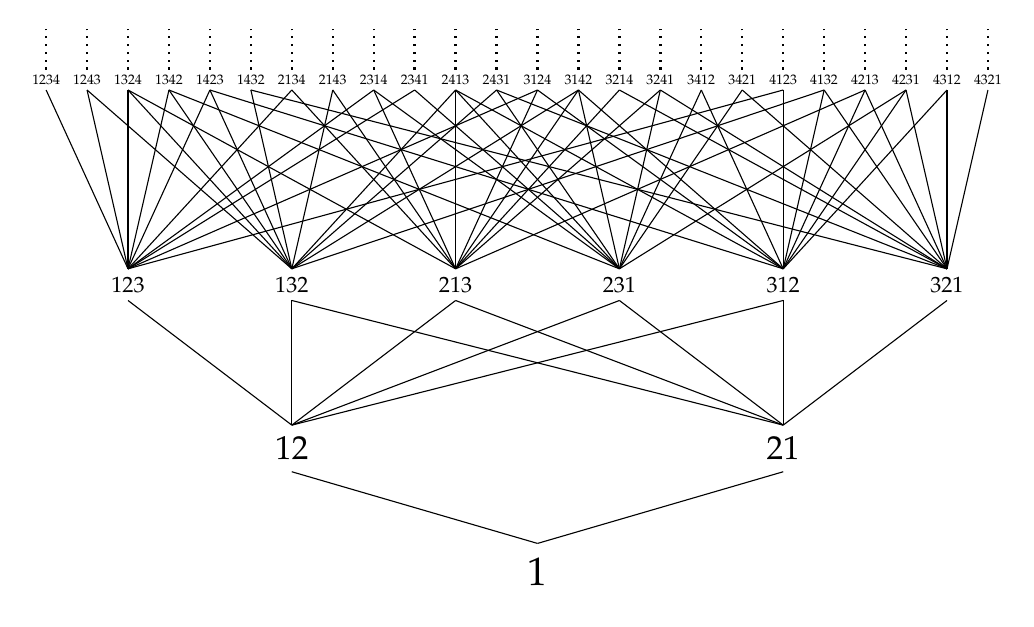
\begin{tikzpicture}[
    every node/.style={},
    scale=.52]
      {\Large
      \node (1) at (12,0) {1};
      }


      {\large
      \node (12) at (6,3) {12};
      \node (21) at (18,3) {21};
      }


      \draw (12.south)-- (1.north);
      \draw (21.south) -- (1.north);


      {\footnotesize
      \node (123) at (2 ,7) {123};
      \node (132) at (6 ,7) {132};
      \node (213) at (10,7) {213};
      \node (231) at (14,7) {231};
      \node (312) at (18,7) {312};
      \node (321) at (22,7) {321};
      }

      \draw (123.south) -- (12.north);
      \draw (132.south) -- (12.north);
      \draw (213.south) -- (12.north);
      \draw (231.south) -- (12.north);
      \draw (312.south) -- (12.north);
      
      \draw (132.south) -- (21.north);
      \draw (213.south) -- (21.north);
      \draw (231.south) -- (21.north);
      \draw (312.south) -- (21.north);
      \draw (321.south) -- (21.north);

      {\tiny
      \node (1234) at (0 ,12) {1234};
      \node (1243) at (1 ,12) {1243};
      \node (1324) at (2 ,12) {1324};
      \node (1342) at (3 ,12) {1342};
      \node (1423) at (4 ,12) {1423};
      \node (1432) at (5 ,12) {1432};

      \node (2134) at (6 ,12) {2134};
      \node (2143) at (7 ,12) {2143};
      \node (2314) at (8 ,12) {2314};
      \node (2341) at (9 ,12) {2341};
      \node (2413) at (10,12) {2413};
      \node (2431) at (11,12) {2431};

      \node (3124) at (12,12) {3124};
      \node (3142) at (13,12) {3142};
      \node (3214) at (14,12) {3214};
      \node (3241) at (15,12) {3241};
      \node (3412) at (16,12) {3412};
      \node (3421) at (17,12) {3421};

      \node (4123) at (18,12) {4123};
      \node (4132) at (19,12) {4132};
      \node (4213) at (20,12) {4213};
      \node (4231) at (21,12) {4231};
      \node (4312) at (22,12) {4312};
      \node (4321) at (23,12) {4321};
      }

      % 123
      \foreach \p in {1234, 1243, 1324, 1342, 1423, 2134, 2314, 2341, 3124, 4123}
        \draw (\p.south) -- (123.north);
      % 132
      \foreach \p in {1243, 1324, 1342, 1423, 1432, 2143, 2413, 2431, 3142, 4132}
        \draw (\p.south) -- (132.north);
      % 213
      \foreach \p in {1324, 2134, 2143, 2314, 2413, 3124, 3142, 3214, 3241, 4213}
        \draw (\p.south) -- (213.north);
      % 231
      \foreach \p in {1342, 2314, 2341, 2413, 2431, 3142, 3241, 3412, 3421, 4231}
        \draw (\p.south) -- (231.north);
      % 312
      \foreach \p in {1423, 2413, 3124, 3142, 3412, 4123, 4132, 4213, 4231, 4312}
        \draw (\p.south) -- (312.north);
      % 321
      \foreach \p in {4321, 3421, 4231, 2431, 3241, 4312, 4132, 1432, 4213, 3214}
        \draw (\p.south) -- (321.north);

      \foreach \p in {1234, 1243, 1324, 1342, 1423, 1432,
                      2134, 2143, 2314, 2341, 2413, 2431,
                      3124, 3142, 3214, 3241, 3412, 3421,
                      4123, 4132, 4213, 4231, 4312, 4321}
        \draw[dotted, line width=.3mm] (\p.north) -- ++(0,1);

    \end{tikzpicture}
  \end{center}
\end{frame}
\restoregeometry


\newgeometry{margin=0mm}
\begin{frame} \frametitle{\hspace{28pt}Permutation Classes - Growth Rates} 
  \begin{center}
    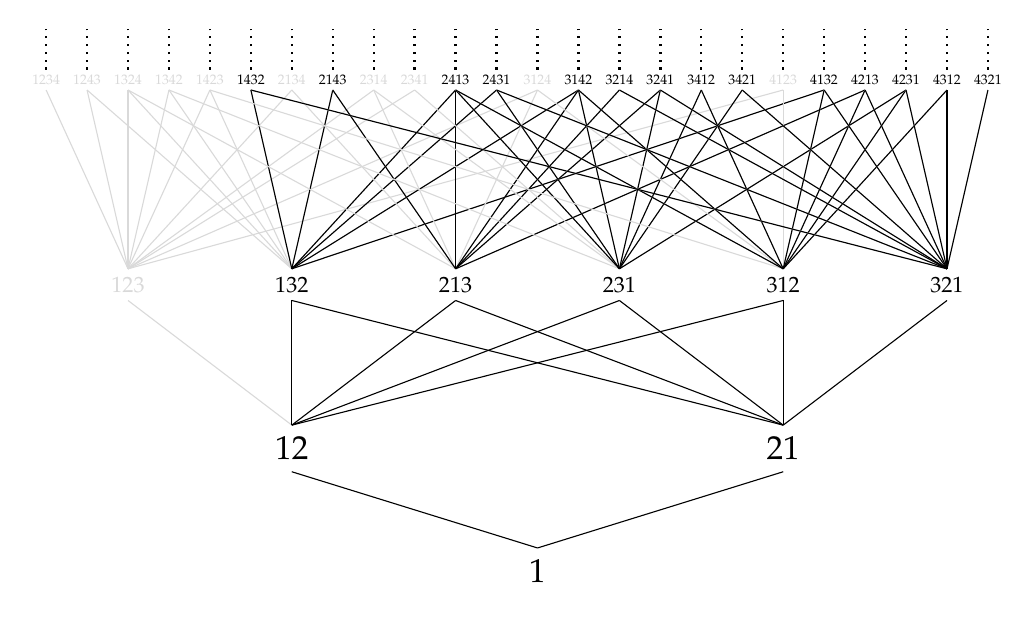
\begin{tikzpicture}[
    every node/.style={},
    scale=.52]

      {\large
      \node (1) at (12,0) {1};
      \node (12) at (6,3) {12};
      \node (21) at (18,3) {21};
      }



      \draw (12.south)-- (1.north);
      \draw (21.south) -- (1.north);


      {\footnotesize
      \node (123) at (2 ,7) {\color{lg}{123}};
      \node (132) at (6 ,7) {132};
      \node (213) at (10,7) {213};
      \node (231) at (14,7) {231};
      \node (312) at (18,7) {312};
      \node (321) at (22,7) {321};
      }

      \draw[color=lg] (123.south) -- (12.north);
      \draw (132.south) -- (12.north);
      \draw (213.south) -- (12.north);
      \draw (231.south) -- (12.north);
      \draw (312.south) -- (12.north);
      
      \draw (132.south) -- (21.north);
      \draw (213.south) -- (21.north);
      \draw (231.south) -- (21.north);
      \draw (312.south) -- (21.north);
      \draw (321.south) -- (21.north);

      {\tiny
      \node (1234) at (0 ,12) {\color{lg}{1234}};
      \node (1243) at (1 ,12) {\color{lg}{1243}};
      \node (1324) at (2 ,12) {\color{lg}{1324}};
      \node (1342) at (3 ,12) {\color{lg}{1342}};
      \node (1423) at (4 ,12) {\color{lg}{1423}};
      \node (1432) at (5 ,12) {1432};

      \node (2134) at (6 ,12) {\color{lg}{2134}};
      \node (2143) at (7 ,12) {2143};
      \node (2314) at (8 ,12) {\color{lg}{2314}};
      \node (2341) at (9 ,12) {\color{lg}{2341}};
      \node (2413) at (10,12) {2413};
      \node (2431) at (11,12) {2431};

      \node (3124) at (12,12) {\color{lg}{3124}};
      % simple:
      \node (3142) at (13,12) {3142};
      %
      \node (3214) at (14,12) {3214};
      \node (3241) at (15,12) {3241};
      \node (3412) at (16,12) {3412};
      \node (3421) at (17,12) {3421};

      \node (4123) at (18,12) {\color{lg}{4123}};
      \node (4132) at (19,12) {4132};
      \node (4213) at (20,12) {4213}; 
      \node (4231) at (21,12) {4231};
      \node (4312) at (22,12) {4312};
      \node (4321) at (23,12) {4321};
      }

      % 123
      \foreach \p in {1234, 1243, 1324, 1342, 1423, 2134, 2314, 2341, 3124, 4123}
        \draw[color=lg] (\p.south) -- (123.north);
      % 132
      \foreach \p in {1243, 1324, 1342, 1423, 1432, 2143, 2413, 2431, 3142, 4132}
        \draw[color=lg] (\p.south) -- (132.north);

      \foreach \p in {1432, 2143, 2413, 2431, 3142, 4132}
        \draw[] (\p.south) -- (132.north);

      % 213
      \foreach \p in {1324, 2134, 2143, 2314, 2413, 3124, 3142, 3214, 3241, 4213}
        \draw[color=lg] (\p.south) -- (213.north);

      \foreach \p in {2143, 2413, 3142, 3214, 3241, 4213}
        \draw[] (\p.south) -- (213.north);

      % 231
      \foreach \p in {1342, 2314, 2341, 2413, 2431, 3142, 3241, 3412, 3421, 4231}
        \draw[color=lg] (\p.south) -- (231.north);

      \foreach \p in {2413, 2431, 3142, 3241, 3412, 3421, 4231}
        \draw[] (\p.south) -- (231.north);

      % 312
      \foreach \p in {1423, 2413, 3124, 3142, 3412, 4123, 4132, 4213, 4231, 4312}
        \draw[color=lg] (\p.south) -- (312.north);

      \foreach \p in {2413, 3142, 3412, 4132, 4213, 4231, 4312}
        \draw[] (\p.south) -- (312.north);

      % 321
      \foreach \p in {4321, 3421, 4231, 2431, 3241, 4312, 4132, 1432, 4213, 3214}
        \draw[color=lg] (\p.south) -- (321.north);

      \foreach \p in {4321, 3421, 4231, 2431, 3241, 4312, 4132, 1432, 4213, 3214}
        \draw[] (\p.south) -- (321.north);


      \foreach \p in {1234, 1243, 1324, 1342, 1423, 1432,
                      2134, 2143, 2314, 2341, 2413, 2431,
                      3124, 3142, 3214, 3241, 3412, 3421,
                      4123, 4132, 4213, 4231, 4312, 4321}
        \draw[dotted, line width=.3mm] (\p.north) -- ++(0,1);

    \end{tikzpicture}
  \end{center}
\end{frame}
\restoregeometry

\newgeometry{margin=0mm}
\begin{frame} \frametitle{\hspace{28pt}Permutation Classes - Growth Rates} 
  \begin{center}
    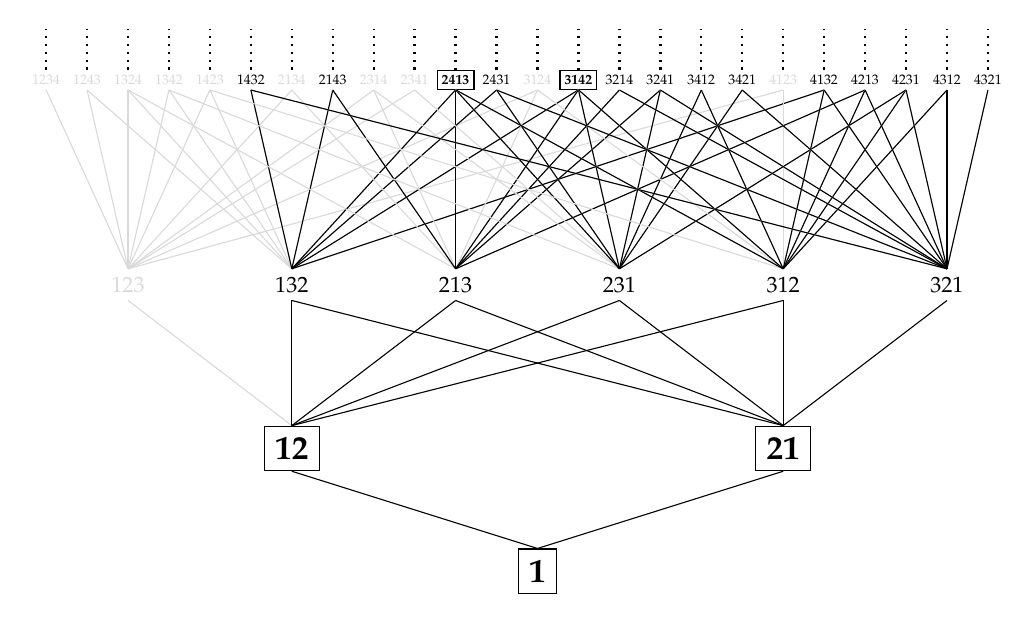
\begin{tikzpicture}[
    every node/.style={},
    scale=.52]

      {\large
      \node[draw=black] (1) at (12,0) {\textbf{1}};
      \node[draw=black] (12) at (6,3) {\textbf{12}};
      \node[draw=black] (21) at (18,3) {\textbf{21}};
      }



      \draw (12.south)-- (1.north);
      \draw (21.south) -- (1.north);


      {\footnotesize
      \node (123) at (2 ,7) {\color{lg}{123}};
      \node (132) at (6 ,7) {132};
      \node (213) at (10,7) {213};
      \node (231) at (14,7) {231};
      \node (312) at (18,7) {312};
      \node (321) at (22,7) {321};
      }

      \draw[color=lg] (123.south) -- (12.north);
      \draw (132.south) -- (12.north);
      \draw (213.south) -- (12.north);
      \draw (231.south) -- (12.north);
      \draw (312.south) -- (12.north);
      
      \draw (132.south) -- (21.north);
      \draw (213.south) -- (21.north);
      \draw (231.south) -- (21.north);
      \draw (312.south) -- (21.north);
      \draw (321.south) -- (21.north);

      {\tiny
      \node (1234) at (0 ,12) {\color{lg}{1234}};
      \node (1243) at (1 ,12) {\color{lg}{1243}};
      \node (1324) at (2 ,12) {\color{lg}{1324}};
      \node (1342) at (3 ,12) {\color{lg}{1342}};
      \node (1423) at (4 ,12) {\color{lg}{1423}};
      \node (1432) at (5 ,12) {1432};

      \node (2134) at (6 ,12) {\color{lg}{2134}};
      \node (2143) at (7 ,12) {2143};
      \node (2314) at (8 ,12) {\color{lg}{2314}};
      \node (2341) at (9 ,12) {\color{lg}{2341}};
      \node[draw=black] (2413) at (10,12) {\textbf{2413}};
      \node (2431) at (11,12) {2431};

      \node (3124) at (12,12) {\color{lg}{3124}};
      \node[draw=black] (3142) at (13,12) {\textbf{3142}};
      \node (3214) at (14,12) {3214};
      \node (3241) at (15,12) {3241};
      \node (3412) at (16,12) {3412};
      \node (3421) at (17,12) {3421};

      \node (4123) at (18,12) {\color{lg}{4123}};
      \node (4132) at (19,12) {4132};
      \node (4213) at (20,12) {4213}; 
      \node (4231) at (21,12) {4231};
      \node (4312) at (22,12) {4312};
      \node (4321) at (23,12) {4321};
      }

      % 123
      \foreach \p in {1234, 1243, 1324, 1342, 1423, 2134, 2314, 2341, 3124, 4123}
        \draw[color=lg] (\p.south) -- (123.north);
      % 132
      \foreach \p in {1243, 1324, 1342, 1423, 1432, 2143, 2413, 2431, 3142, 4132}
        \draw[color=lg] (\p.south) -- (132.north);

      \foreach \p in {1432, 2143, 2413, 2431, 3142, 4132}
        \draw[] (\p.south) -- (132.north);

      % 213
      \foreach \p in {1324, 2134, 2143, 2314, 2413, 3124, 3142, 3214, 3241, 4213}
        \draw[color=lg] (\p.south) -- (213.north);

      \foreach \p in {2143, 2413, 3142, 3214, 3241, 4213}
        \draw[] (\p.south) -- (213.north);

      % 231
      \foreach \p in {1342, 2314, 2341, 2413, 2431, 3142, 3241, 3412, 3421, 4231}
        \draw[color=lg] (\p.south) -- (231.north);

      \foreach \p in {2413, 2431, 3142, 3241, 3412, 3421, 4231}
        \draw[] (\p.south) -- (231.north);

      % 312
      \foreach \p in {1423, 2413, 3124, 3142, 3412, 4123, 4132, 4213, 4231, 4312}
        \draw[color=lg] (\p.south) -- (312.north);

      \foreach \p in {2413, 3142, 3412, 4132, 4213, 4231, 4312}
        \draw[] (\p.south) -- (312.north);

      % 321
      \foreach \p in {4321, 3421, 4231, 2431, 3241, 4312, 4132, 1432, 4213, 3214}
        \draw[color=lg] (\p.south) -- (321.north);

      \foreach \p in {4321, 3421, 4231, 2431, 3241, 4312, 4132, 1432, 4213, 3214}
        \draw[] (\p.south) -- (321.north);


      \foreach \p in {1234, 1243, 1324, 1342, 1423, 1432,
                      2134, 2143, 2314, 2341, 2413, 2431,
                      3124, 3142, 3214, 3241, 3412, 3421,
                      4123, 4132, 4213, 4231, 4312, 4321}
        \draw[dotted, line width=.3mm] (\p.north) -- ++(0,1);

    \end{tikzpicture}
  \end{center}
\end{frame}
\restoregeometry

\begin{frame}{How Rare are Simples?}
  \pause
  \begin{block}{Theorem (Albert, Atkinson, Klazar)}
    A randomly chosen permutation is simple with probability $1/e^2$.  
  \end{block}

  \pause
  \begin{block}{However\dots}
    There is no known instance of a permutation class' simples having positive 
    density.
  \end{block}
\end{frame}

\begin{frame}{Deflatability}
  \begin{block}{The Simple Subclass}
    Within a class of permutations, define the \emph{simple subclass} to be the 
    smallest subclass which contains all the simple permutations of the class.
  \end{block}
  \pause
  \begin{block}{Deflatable Classes}
    A class is \emph{deflatable} if its simple subclass is strictly smaller than 
    the class itself. 
  \end{block}
\end{frame}

\begin{frame}{Deflatability}
  \pause
  \begin{center}
  \begin{tikzpicture}[scale=.85]
    \begin{pgfonlayer}{bg}
    \draw[fill = black!5, draw = none] (0,0) -- (-6,6) -- (6,6) -- cycle;
    \end{pgfonlayer}
    \draw[thick] (-6,6) -- (0,0) -- (6,6);
    \only<3->{
      \draw[fill=black] (-0.92, 2.20) circle (.3mm);
      \draw[fill=black] (-1.15, 4.63) circle (.3mm);
      \draw[fill=black] (0.25, 0.95) circle (.3mm);
      \draw[fill=black] (-0.72, 3.06) circle (.3mm);
      \draw[fill=black] (0.03, 1.79) circle (.3mm);
      \draw[fill=black] (0.00, 1.05) circle (.3mm);
      \draw[fill=black] (-0.97, 5.30) circle (.3mm);
      \draw[fill=black] (-0.02, 0.70) circle (.3mm);
      \draw[fill=black] (-0.33, 3.68) circle (.3mm);
      \draw[fill=black] (-0.47, 2.81) circle (.3mm);
      \draw[fill=black] (0.41, 1.66) circle (.3mm);
      \draw[fill=black] (-0.45, 1.15) circle (.3mm);
      \draw[fill=black] (-1.13, 4.06) circle (.3mm);
      \draw[fill=black] (-0.71, 1.62) circle (.3mm);
      \draw[fill=black] (0.49, 3.02) circle (.3mm);
      \draw[fill=black] (0.26, 0.81) circle (.3mm);
      \draw[fill=black] (-0.16, 0.62) circle (.3mm);
      \draw[fill=black] (-0.11, 3.55) circle (.3mm);
      \draw[fill=black] (2.63, 5.42) circle (.3mm);
      \draw[fill=black] (0.13, 1.31) circle (.3mm);
      \draw[fill=black] (2.23, 5.35) circle (.3mm);
      \draw[fill=black] (0.59, 1.44) circle (.3mm);
      \draw[fill=black] (0.15, 0.53) circle (.3mm);
      \draw[fill=black] (1.26, 3.67) circle (.3mm);
      \draw[fill=black] (-0.75, 3.93) circle (.3mm);
      \draw[fill=black] (-0.10, 0.64) circle (.3mm);
      \draw[fill=black] (0.19, 0.98) circle (.3mm);
      \draw[fill=black] (-2.69, 5.40) circle (.3mm);
      \draw[fill=black] (-0.03, 1.45) circle (.3mm);
      \draw[fill=black] (-1.97, 4.61) circle (.3mm);
      \draw[fill=black] (-0.36, 0.93) circle (.3mm);
      \draw[fill=black] (-0.09, 4.21) circle (.3mm);
      \draw[fill=black] (-0.57, 3.76) circle (.3mm);
      \draw[fill=black] (1.36, 5.39) circle (.3mm);
      \draw[fill=black] (0.19, 1.85) circle (.3mm);
      \draw[fill=black] (-0.42, 1.84) circle (.3mm);
      \draw[fill=black] (0.33, 4.37) circle (.3mm);
      \draw[fill=black] (0.93, 3.32) circle (.3mm);
      \draw[fill=black] (-1.09, 3.89) circle (.3mm);
      \draw[fill=black] (-1.26, 4.32) circle (.3mm);
      \draw[fill=black] (1.72, 3.97) circle (.3mm);
      \draw[fill=black] (0.51, 1.32) circle (.3mm);
      \draw[fill=black] (1.22, 4.25) circle (.3mm);
      \draw[fill=black] (1.40, 3.12) circle (.3mm);
      \draw[fill=black] (0.79, 2.31) circle (.3mm);
      \draw[fill=black] (1.45, 4.72) circle (.3mm);
      \draw[fill=black] (-0.34, 1.02) circle (.3mm);
      \draw[fill=black] (0.59, 4.41) circle (.3mm);
      \draw[fill=black] (1.13, 3.77) circle (.3mm);
      \draw[fill=black] (-1.49, 4.48) circle (.3mm);
      \draw[fill=black] (0.11, 2.56) circle (.3mm);
      \draw[fill=black] (-2.21, 4.53) circle (.3mm);
      \draw[fill=black] (-0.41, 2.16) circle (.3mm);
      \draw[fill=black] (1.39, 4.32) circle (.3mm);
      \draw[fill=black] (-1.08, 4.04) circle (.3mm);
      \draw[fill=black] (-0.06, 2.17) circle (.3mm);
      \draw[fill=black] (-2.12, 4.26) circle (.3mm);
      \draw[fill=black] (0.22, 1.45) circle (.3mm);
      \draw[fill=black] (-1.75, 4.50) circle (.3mm);
      \draw[fill=black] (-0.67, 1.68) circle (.3mm);
      \draw[fill=black] (-0.41, 2.80) circle (.3mm);
      \draw[fill=black] (1.04, 4.20) circle (.3mm);
      \draw[fill=black] (1.02, 4.40) circle (.3mm);
      \draw[fill=black] (-0.60, 2.00) circle (.3mm);
      \draw[fill=black] (0.67, 3.64) circle (.3mm);
      \draw[fill=black] (-1.12, 3.68) circle (.3mm);
      \draw[fill=black] (-0.11, 3.94) circle (.3mm);
      \draw[fill=black] (0.25, 3.28) circle (.3mm);
      \draw[fill=black] (0.00, 0.66) circle (.3mm);
      \draw[fill=black] (0.62, 3.39) circle (.3mm);
      \draw[fill=black] (0.13, 4.89) circle (.3mm);
      \draw[fill=black] (-0.11, 1.29) circle (.3mm);
      \draw[fill=black] (0.51, 2.43) circle (.3mm);
      \draw[fill=black] (0.16, 1.39) circle (.3mm);
      \draw[fill=black] (2.07, 4.48) circle (.3mm);
      \draw[fill=black] (1.44, 3.42) circle (.3mm);
      \draw[fill=black] (-0.30, 2.26) circle (.3mm);
      \draw[fill=black] (0.18, 3.52) circle (.3mm);
      \draw[fill=black] (1.17, 3.22) circle (.3mm);
      \draw[fill=black] (0.53, 4.93) circle (.3mm);
      \draw[fill=black] (1.58, 4.97) circle (.3mm);
      \draw[fill=black] (0.47, 1.78) circle (.3mm);
      \draw[fill=black] (0.42, 0.97) circle (.3mm);
      \draw[fill=black] (0.14, 0.75) circle (.3mm);
      \draw[fill=black] (1.97, 5.21) circle (.3mm);
      \draw[fill=black] (-0.70, 3.63) circle (.3mm);
      \draw[fill=black] (-1.18, 4.86) circle (.3mm);
      \draw[fill=black] (0.44, 1.23) circle (.3mm);
      \draw[fill=black] (0.48, 4.64) circle (.3mm);
      \draw[fill=black] (-0.88, 2.80) circle (.3mm);
      \draw[fill=black] (1.10, 4.23) circle (.3mm);
      \draw[fill=black] (-0.10, 1.43) circle (.3mm);
      \draw[fill=black] (-0.51, 5.08) circle (.3mm);
      \draw[fill=black] (-0.62, 3.47) circle (.3mm);
      \draw[fill=black] (0.53, 3.54) circle (.3mm);
      \draw[fill=black] (0.06, 1.82) circle (.3mm);
      \draw[fill=black] (0.01, 1.85) circle (.3mm);
      \draw[fill=black] (-0.07, 0.83) circle (.3mm);
      \draw[fill=black] (-0.29, 1.94) circle (.3mm);
      \draw[fill=black] (-0.30, 5.47) circle (.3mm);
    }
    \only<4>{
    \begin{pgfonlayer}{bg}
      \draw[fill = black!20, draw = none] (0,0) -- (-3,6) -- (3,6) -- cycle;
    \end{pgfonlayer}
    \draw[thick] (-3,6) -- (0,0) -- (3,6);
    }
  \end{tikzpicture}
  \end{center}
\end{frame}

\begin{frame}{Deflatability}
  \begin{block}{Alternate Definition}
    A permutation class is deflatable if the downward closure of its simples is 
    strictly smaller than the class itself. \\[1pc]
    \pause
    A permutation class $C$ is \emph{not} deflatable if every permutation in the 
    class is contained within a simple permutation in the class. 
  \end{block}
\end{frame}

\begin{frame}{Proving Non-Deflatability}
  \pause
  \begin{block}{Idea}
    Let $\C$ be a class. Given an arbitrary permutation $\omega$ in $\C$, we 
    need to show that $\omega$ can be \emph{extended} to a simple permutation 
    within the class. 
  \end{block}
  \pause
  \begin{block}{Lemma}
    Every permutation in $\Av(\pi)$ can be extended to an indecomposable 
    permutation (within the class), except when $\pi \in \{1, 12, 21, 132, 213, 
    231, 312\}$. 
  \end{block}
  \pause
  \begin{block}{Lemma}
    A permutation class $\Av(\pi)$ is deflatable if, for every $\omega \in 
    \Av(\pi)$, we can extend $\omega$ by a single point which \emph{cuts} a 
    maximal interval of $\omega$. 
  \end{block}

\end{frame}


\begin{frame}{Proving Non-Deflatability}
      \begin{center}
			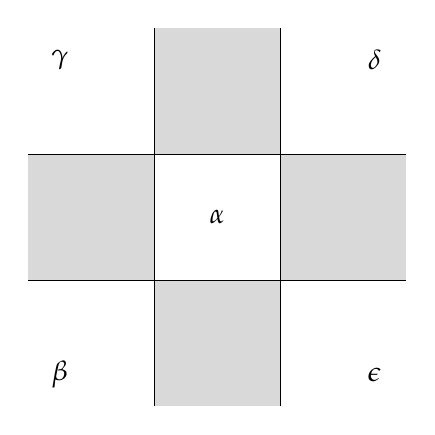
\begin{tikzpicture}[scale = .8]
				\draw[draw=none, fill=black!15] (2,0) rectangle ++(2,2);
				\draw[draw=none, fill=black!15] (0,2) rectangle ++(2,2);
				\draw[draw=none, fill=black!15] (2,4) rectangle ++(2,2);
				\draw[draw=none, fill=black!15] (4,2) rectangle ++(2,2);
				\foreach \i in {2,4} {
					\draw (\i,0) -- (\i,6);
					\draw (0,\i) -- (6,\i);
				}
				\node at (3,3) {$\alpha$};
				\node at (.5,5.5) {$\gamma$};
				\node at (.5,.5) {$\beta$};
				\node at (5.5,.5) {$\epsilon$};
				\node at (5.5,5.5) {$\delta$};
			\end{tikzpicture}
      \end{center}
\end{frame}


\begin{frame}{The Class $\Av(2413)$}
  \begin{block}{Theorem}
    The class $\Av(2413)$ is non-deflatable
  \end{block}
  \pause
  \begin{block}{Proof}
    Let $\omega \in \Av(2413)$ be indecomposable and non-simple, and let 
    $\alpha$ be a maximal interval. We need to add a point to $\omega$ which 
    cuts $\alpha$ without creating an occurrence of $2413$. 
  \end{block}
\end{frame}
    

\begin{frame}{The Class $\Av(2413)$}
      \only<1>{
      \begin{center}
			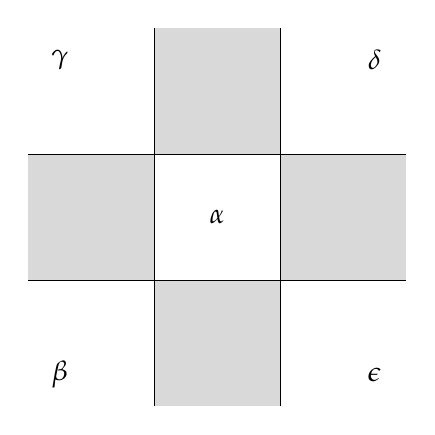
\begin{tikzpicture}[scale = .8]
				\draw[draw=none, fill=black!15] (2,0) rectangle ++(2,2);
				\draw[draw=none, fill=black!15] (0,2) rectangle ++(2,2);
				\draw[draw=none, fill=black!15] (2,4) rectangle ++(2,2);
				\draw[draw=none, fill=black!15] (4,2) rectangle ++(2,2);
				\foreach \i in {2,4} {
					\draw (\i,0) -- (\i,6);
					\draw (0,\i) -- (6,\i);
				}
				\node at (3,3) {$\alpha$};
				\node at (.5,5.5) {$\gamma$};
				\node at (.5,.5) {$\beta$};
				\node at (5.5,.5) {$\epsilon$};
				\node at (5.5,5.5) {$\delta$};
			\end{tikzpicture}
      \end{center}
      }\only<2>{
      \begin{center}
			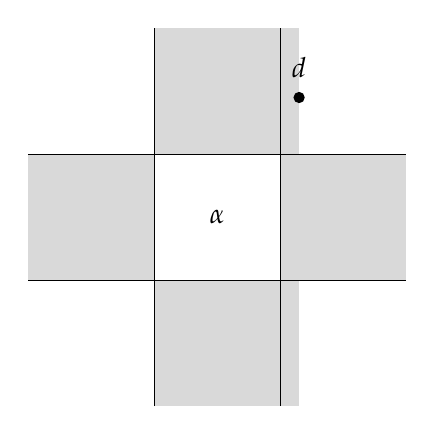
\begin{tikzpicture}[scale = .8]
				\draw[draw=none, fill=black!15] (2,0) rectangle ++(2.3,2);
				\draw[draw=none, fill=black!15] (0,2) rectangle ++(2,2);
				\draw[draw=none, fill=black!15] (2,4) rectangle ++(2.3,2);
				\draw[draw=none, fill=black!15] (4,2) rectangle ++(2,2);
				\foreach \i in {2,4} {
					\draw (\i,0) -- (\i,6);
					\draw (0,\i) -- (6,\i);
				}
				\node at (3,3) {$\alpha$};
				\draw[fill=black] (4.3, 4.9) circle (.08) node[label=above:$d$] (d) {};
			\end{tikzpicture}
      \end{center}
      }\only<3>{
      \begin{center}
			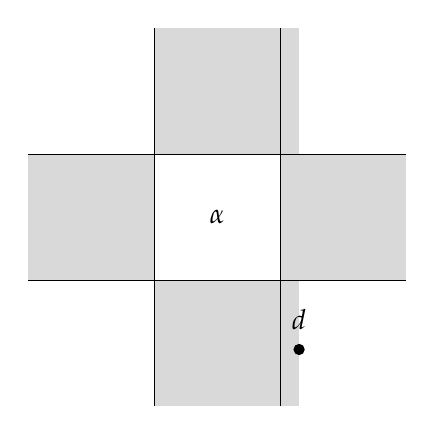
\begin{tikzpicture}[scale = .8]
				\draw[draw=none, fill=black!15] (2,0) rectangle ++(2.3,2);
				\draw[draw=none, fill=black!15] (0,2) rectangle ++(2,2);
				\draw[draw=none, fill=black!15] (2,4) rectangle ++(2.3,2);
				\draw[draw=none, fill=black!15] (4,2) rectangle ++(2,2);
				\foreach \i in {2,4} {
					\draw (\i,0) -- (\i,6);
					\draw (0,\i) -- (6,\i);
				}
				\node at (3,3) {$\alpha$};
				\draw[fill=black] (4.3, .9) circle (.08) node[label=above:$d$] (d) {};
			\end{tikzpicture}
      \end{center}
      }\only<4>{
      \begin{center}
			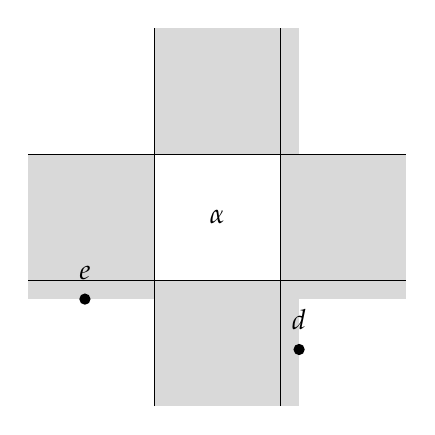
\begin{tikzpicture}[scale = .8]
				\draw[draw=none, fill=black!15] (2,0) rectangle ++(2.3,2);
				\draw[draw=none, fill=black!15] (0,1.7) rectangle ++(2,2.3);
				\draw[draw=none, fill=black!15] (2,4) rectangle ++(2.3,2);
				\draw[draw=none, fill=black!15] (4,1.7) rectangle ++(2,2.3);
				\foreach \i in {2,4} {
					\draw (\i,0) -- (\i,6);
					\draw (0,\i) -- (6,\i);
				}
				\node at (3,3) {$\alpha$};
				\draw[fill=black] (4.3, .9) circle (.08) node[label=above:$d$] (d) {};
				\draw[fill=black] (.9, 1.7) circle (.08) node[label=above:$e$] (e) {};
			\end{tikzpicture}
      \end{center}
      }\only<5>{
      \begin{center}
			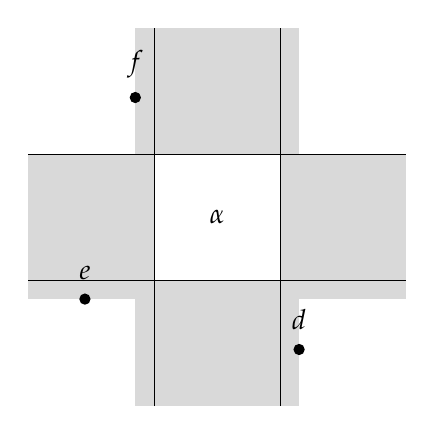
\begin{tikzpicture}[scale = .8]
				\draw[draw=none, fill=black!15] (1.7,0) rectangle ++(2.6,2);
				\draw[draw=none, fill=black!15] (0,1.7) rectangle ++(2,2.3);
				\draw[draw=none, fill=black!15] (1.7,4) rectangle ++(2.6,2);
				\draw[draw=none, fill=black!15] (4,1.7) rectangle ++(2,2.3);
				\foreach \i in {2,4} {
					\draw (\i,0) -- (\i,6);
					\draw (0,\i) -- (6,\i);
				}
				\node at (3,3) {$\alpha$};
				\draw[fill=black] (4.3, .9) circle (.08) node[label=above:$d$] (d) {};
				\draw[fill=black] (.9, 1.7) circle (.08) node[label=above:$e$] (e) {};
				\draw[fill=black] (1.7, 4.9) circle (.08) node[label=above:$f$] (f) {};
			\end{tikzpicture}
      \end{center}
      }\only<6>{
      \begin{center}
			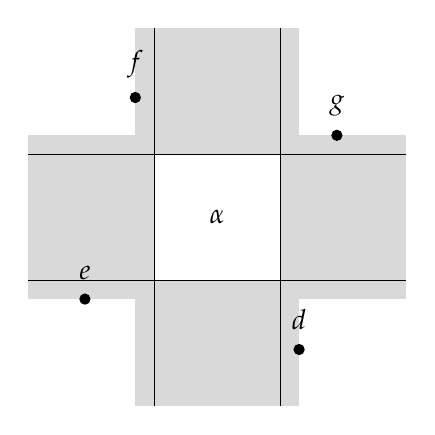
\begin{tikzpicture}[scale = .8]
				\draw[draw=none, fill=black!15] (1.7,0) rectangle ++(2.6,2);
				\draw[draw=none, fill=black!15] (0,1.7) rectangle ++(2,2.6);
				\draw[draw=none, fill=black!15] (1.7,4) rectangle ++(2.6,2);
				\draw[draw=none, fill=black!15] (4,1.7) rectangle ++(2,2.6);
				\foreach \i in {2,4} {
					\draw (\i,0) -- (\i,6);
					\draw (0,\i) -- (6,\i);
				}
				\node at (3,3) {$\alpha$};
				\draw[fill=black] (4.3, .9) circle (.08) node[label=above:$d$] (d) {};
				\draw[fill=black] (.9, 1.7) circle (.08) node[label=above:$e$] (e) {};
				\draw[fill=black] (1.7, 4.9) circle (.08) node[label=above:$f$] (f) {};
				\draw[fill=black] (4.9, 4.3) circle (.08) node[label=above:$g$] (g) {};
			\end{tikzpicture}
      \end{center}
      }\only<7>{
      \begin{center}
			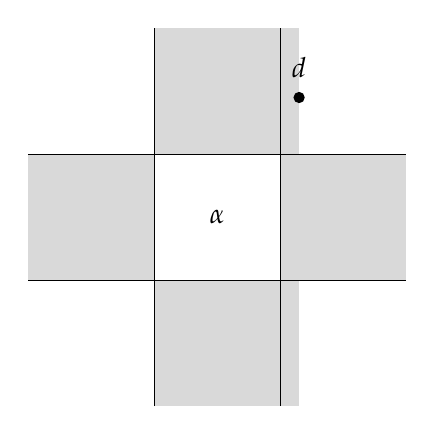
\begin{tikzpicture}[scale = .8]
				\draw[draw=none, fill=black!15] (2,0) rectangle ++(2.3,2);
				\draw[draw=none, fill=black!15] (0,2) rectangle ++(2,2);
				\draw[draw=none, fill=black!15] (2,4) rectangle ++(2.3,2);
				\draw[draw=none, fill=black!15] (4,2) rectangle ++(2,2);
				\foreach \i in {2,4} {
					\draw (\i,0) -- (\i,6);
					\draw (0,\i) -- (6,\i);
				}
				\node at (3,3) {$\alpha$};
				\draw[fill=black] (4.3, 4.9) circle (.08) node[label=above:$d$] (d) {};
			\end{tikzpicture}
      \end{center}
      }\only<8>{
      \begin{center}
			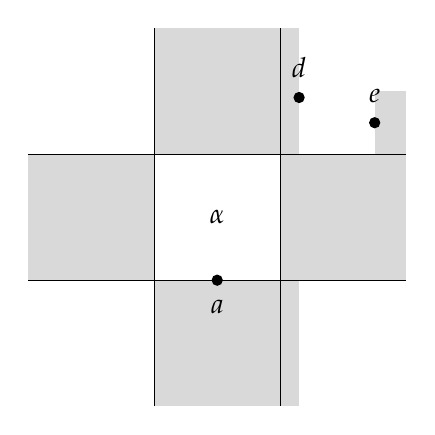
\begin{tikzpicture}[scale = .8]
				\draw[draw=none, fill=black!15] (2,0) rectangle ++(2.3,2);
				\draw[draw=none, fill=black!15] (0,2) rectangle ++(2,2);
				\draw[draw=none, fill=black!15] (2,4) rectangle ++(2.3,2);
				\draw[draw=none, fill=black!15] (4,2) rectangle ++(2,2);
        \draw[draw=none, fill=black!15] (5.5, 4) rectangle ++(.5,1);
				\foreach \i in {2,4} {
					\draw (\i,0) -- (\i,6);
					\draw (0,\i) -- (6,\i);
				}
				\node at (3,3) {$\alpha$};
				\draw[fill=black] (4.3, 4.9) circle (.08) node[label=above:$d$] (d) {};
				\draw[fill=black] (5.5, 4.5) circle (.08) node[label=above:$e$] (e) {};
				\draw[fill=black] (3, 2) circle (.08) node[label=below:$a$] (a) {};
			\end{tikzpicture}
      \end{center}
      }\only<9->{
      \begin{center}
			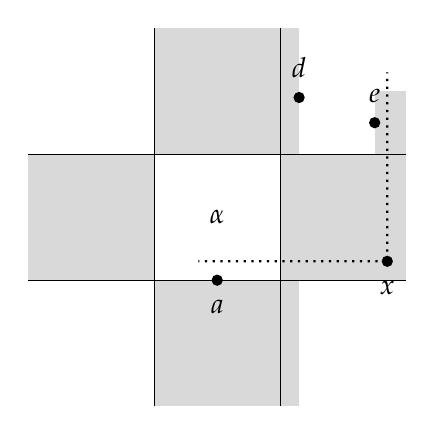
\begin{tikzpicture}[scale = .8]
				\draw[draw=none, fill=black!15] (2,0) rectangle ++(2.3,2);
				\draw[draw=none, fill=black!15] (0,2) rectangle ++(2,2);
				\draw[draw=none, fill=black!15] (2,4) rectangle ++(2.3,2);
				\draw[draw=none, fill=black!15] (4,2) rectangle ++(2,2);
        \draw[draw=none, fill=black!15] (5.5, 4) rectangle ++(.5,1);
				\foreach \i in {2,4} {
					\draw (\i,0) -- (\i,6);
					\draw (0,\i) -- (6,\i);
				}
				\node at (3,3) {$\alpha$};
				\draw[fill=black] (4.3, 4.9) circle (.08) node[label=above:$d$] (d) {};
				\draw[fill=black] (5.5, 4.5) circle (.08) node[label=above:$e$] (e) {};
				\draw[fill=black] (3, 2) circle (.08) node[label=below:$a$] (a) {};
				\draw[fill=black] (5.7, 2.3) circle (.08) node[label=below:$x$] (x) {};

        \draw[dotted, thick] (x) -- ++(-3,0);
        \draw[dotted, thick] (x) -- ++(0,3);
			\end{tikzpicture}
      \end{center}
       }

       \uncover<10>{
       Now claim that this new permutatation avoids 2413
       }
\end{frame}

\begin{frame}{Non-Deflatable Classes}
  \begin{block}{Theorem}
    The class $\Av(\pi)$ is not deflatable whenever \dots
    \begin{itemize}
    \pause
    \item $\pi = \lambda \oplus \mu \oplus \rho$, all three summands non-empty
    \pause
    \item $\pi = \lambda \oplus \rho$, $|\lambda|, |\rho| \geq 2$
    \pause
    \item $\pi = 1 \oplus \rho$, and $\rho$ begins with ascent and lacks either 
    an increasing or a decreasing bond. 
    \pause
    \item $\pi = 1 \oplus \rho$, and $\rho$ ends with its smallest element and does 
    not start with its biggest or second smallest
    \pause
    \item $\pi = 1 \oplus \rho$, and $\rho$ begins with its largest entry and 
    ends with its smallest, and lacks either an increasing or a decreasing bond
    \pause
    \item $\pi = 1 \oplus \rho$, and $\rho$ starts with a descent, has at least 
    one entry to the right of its smallest which is less than its leftmost, and 
    lacks either an increasing or a decreasing bond
    \end{itemize}
  \end{block}
\end{frame}

\begin{frame}{Non-Deflatable Classes}
  \begin{block}{What we've shown}
    For \emph{most} decomposable patterns $\pi$, the class $\Av(\pi)$ is not 
    deflatable. 

    The only (possible) exceptions all have the form $1 \oplus \rho$, with 
    strict restrictions on $\rho$. 
  \end{block}

  \pause

  \begin{block}{$\Av(132)$}
    Recall that $\Av(132)$ is (very) deflatable.
    \pause

    The class $\Av(134652)$ is as well.
  \end{block}

  \pause
  
  \begin{block}{Unknown}
    \begin{itemize}
    \item $\Av(146523)$
    \item $\Av(154623)$
    \item $\Av(164532)$
    \end{itemize}
  \end{block}
\end{frame}




\begin{frame}{Deflatable Classes}
  \pause
  \begin{block}{Idea}
    To prove that a class is deflatable, we need only provide a single 
    \emph{witness}, a permutation in the class which cannot be extended to a 
    simple permutation. 
  \end{block}
\end{frame}


\begin{frame}{Witnessing Deflation}
  Let $\omega \in \Av(\pi)$, and consider the permutation diagram of $\omega$. 
  Denote by gray the \emph{forbidden areas} (those for which inserting an entry 
  creates an occurrence of $\pi$).  \\
  While adding points to $\omega$, if you ever find yourself in this situation:
  \begin{center}
  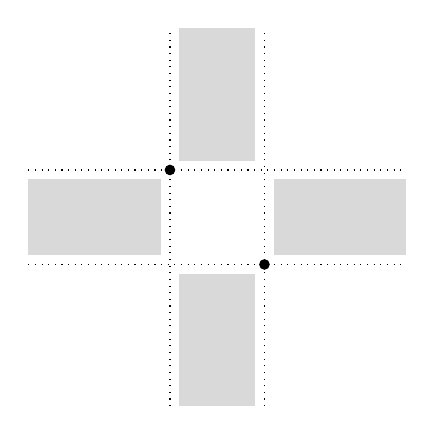
\begin{tikzpicture}[scale=.6]
    \draw[draw = none] (0,0) rectangle (8,8);
    \foreach \i in {3,5}{
      \draw[dotted] (0, \i) -- (8, \i);
      \draw[dotted] (\i, 0) -- (\i, 8);
    }
    \draw[draw = none, fill = black!15] (3.2, 0) rectangle (4.8, 2.8);
    \draw[draw = none, fill = black!15] (3.2, 5.2) rectangle (4.8, 8);
    \draw[draw = none, fill = black!15] (0, 3.2) rectangle (2.8, 4.8);
    \draw[draw = none, fill = black!15] (5.2, 3.2) rectangle (8, 4.8);

    \draw[fill=black] (3,5) circle (1mm);
    \draw[fill=black] (5,3) circle (1mm);

  \end{tikzpicture}
  \end{center}

  Then $\omega$ can never be extended to a simple permutation.
\end{frame}


\begin{frame}{A Deflatable Class}
  \begin{block}{Example}
    The class $\Av(251364)$ is deflatable, as evidenced by the witness $\omega = 
    25173486$.
  \end{block}
  \pause
  \begin{center}
  \begin{tikzpicture}[scale = .5,
                      dot/.style={circle, fill=teal, inner sep=.5mm}]
    \foreach \y [count = \x] in {2,5,1,3,6,4}{
      \node[dot] at (\x,\y) {};
    }
    \node at (3,-2) {$\pi = 251364$};
    \draw[dotted] (0,0) rectangle (7,7);
  \end{tikzpicture}
  \hspace{2pc}
  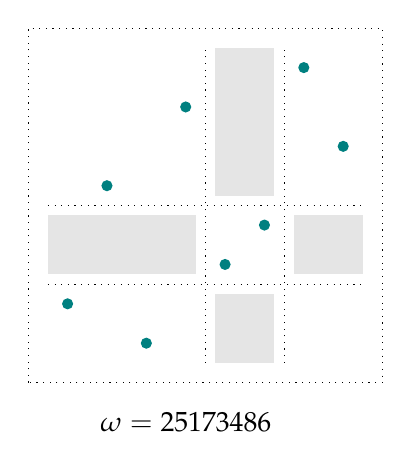
\begin{tikzpicture}[scale = .5,
                      dot/.style={circle, fill=teal, inner sep=.5mm}]
    \foreach \y [count = \x] in {2,5,1,7,3,4,8,6}{
      \node[dot] at (\x,\y) {};
    }
    \node at (4,-1) {$\omega = 25173486$};
    \draw[dotted] (0,0) rectangle (9,9);

    \uncover<3->{
      \draw[dotted] (.5, 2.5) -- (8.5,2.5);
      \draw[dotted] (.5, 4.5) -- (8.5,4.5);
      \draw[dotted] (4.5, .5) -- (4.5,8.5);
      \draw[dotted] (6.5, .5) -- (6.5,8.5);
    }

    \uncover<4>{
      \draw[draw=none, fill=black!10] (.5, 2.75) rectangle (4.25, 4.25);
      \draw[draw=none, fill=black!10] (4.75, .5) rectangle (6.25, 2.25);
      \draw[draw=none, fill=black!10] (6.75, 2.75) rectangle (8.5, 4.25);
      \draw[draw=none, fill=black!10] (4.75, 4.75) rectangle (6.25, 8.5);
    }
    \end{tikzpicture}
    \end{center}
\end{frame}


\begin{frame}{Infinitely Many Deflatable Classes}
  \begin{block}{Theorem}
    Let $\pi = 251364$ and $\theta$ be any permutation. Then the class 
    $\Av(\pi[1,\theta,1,1,1,1])$ is deflatable, as evidenced by the witness $\omega = 
    25173486[1,\theta,1,\theta,1,1,1,1]$.
  \end{block}
  \pause
  \begin{center}
  \begin{tikzpicture}[scale = .5,
                      dot/.style={circle, fill=teal, inner sep=.5mm}]
    \foreach \y [count = \x] in {2,5,1,3,6,4}{
      \node[dot] at (\x,\y) {};
    }
    \node at (3,-2) {$\pi = 251364$};
    \draw[dotted] (0,0) rectangle (7,7);
    \node[draw, rectangle, fill=white] at (2,5) {$\theta$};
  \end{tikzpicture}
  \hspace{2pc}
  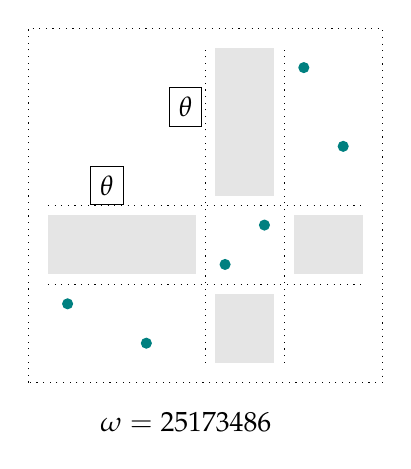
\begin{tikzpicture}[scale = .5,
                      dot/.style={circle, fill=teal, inner sep=.5mm}]
    \foreach \y [count = \x] in {2,5,1,7,3,4,8,6}{
      \node[dot] at (\x,\y) {};
    }
    \node at (4,-1) {$\omega = 25173486$};
    \draw[dotted] (0,0) rectangle (9,9);
    \node[draw, rectangle, fill=white] at (2,5) {$\theta$};
    \node[draw, rectangle, fill=white] at (4,7) {$\theta$};

    \uncover<3->{
      \draw[dotted] (.5, 2.5) -- (8.5,2.5);
      \draw[dotted] (.5, 4.5) -- (8.5,4.5);
      \draw[dotted] (4.5, .5) -- (4.5,8.5);
      \draw[dotted] (6.5, .5) -- (6.5,8.5);
    }

    \uncover<4>{
      \draw[draw=none, fill=black!10] (.5, 2.75) rectangle (4.25, 4.25);
      \draw[draw=none, fill=black!10] (4.75, .5) rectangle (6.25, 2.25);
      \draw[draw=none, fill=black!10] (6.75, 2.75) rectangle (8.5, 4.25);
      \draw[draw=none, fill=black!10] (4.75, 4.75) rectangle (6.25, 8.5);
    }
    \end{tikzpicture}
    \end{center}
\end{frame}

\begin{frame}{More Deflatable Classes}
  \pause
  {\footnotesize
    \rowcolors{2}{teal!0}{teal!10}
  \begin{tabular}{cc}
  Class & Witness \\ 
		$\Av(134652)$ & $6\;8\;9\;3\;4\;1\;10\;14\;7\;13\;5\;12\;11\;2$\\
		$\Av(246135)$ & $4\;7\;2\;9\;11\;5\;6\;1\;10\;3\;8$\\
		$\Av(246513)$ & $5\;9\;3\;11\;8\;2\;10\;6\;7\;1\;4$\\
		$\Av(251364)$ & $2\;5\;1\;7\;3\;4\;8\;6$\\
		$\Av(251463)$ & $2\;6\;1\;8\;4\;3\;7\;9\;5$\\
		$\Av(254613)$ & $5\;9\;3\;11\;2\;8\;10\;6\;7\;1\;4$\\
		$\Av(256413)$ & $4\;7\;9\;2\;10\;8\;5\;6\;1\;3$\\
		$\Av(1523764)$ & $11\;18\;14\;16\;8\;19\;6\;7\;22\;13\;1\;10\;5\;24\;2\;3\;9\;17\;23\;4\;21\;20\;15\;12$\\
		$\Av(2613475)$ & $2\;6\;1\;3\;9\;4\;5\;7\;10\;8$\\
		$\Av(2631574)$ & $2\;6\;3\;1\;9\;5\;4\;8\;10\;7$\\
  \end{tabular}
  }


\end{frame}

\begin{frame}{What's Left?}
  \pause
  \begin{block}{Open Questions} 
    Are the following classes deflatable?
  \end{block}
  \pause
  \begin{minipage}{.45\framewidth}
  \begin{block}{Decomposable Bases}
    \begin{itemize}
      \item $\Av(146523)$
      \item $\Av(154623)$
      \item $\Av(164532)$
    \end{itemize}
  \end{block}
  \end{minipage}
  \pause
  \begin{minipage}{.45\framewidth}
  \begin{block}{Indecomposable Bases}
    \begin{itemize}
      \item $\Av(25314)$
      \item $\Av(24153)$
      \item $\Av(23514)$
      \item $\Av(24513)$
    \end{itemize}
  \end{block}
  \end{minipage}
  \pause
  \begin{block}{Conjecture}
    If $\pi$ is a \emph{parallel alternation} of length $\geq 6$ (i.e., $\pi = 
    246\dots (2n) 135 \dots (2n-1)$), then the class $\Av(\pi)$ is deflatable.
  \end{block}
\end{frame}



\end{document}

